\chapter{绪\hskip 0.4cm 论}
\label{ch1}

\section{研究背景}
在过去的近十年,人工智能(Artificial Intelligence,AI)取得了令人难以置信的进步,广泛地应用于各种领域。为了进一步提高模型的训练精度和学习能力,新兴的深度神经网络,也称为深度学习(Deep Learning,DL)随之提出,深度学习凭借其高效的数据建模、抽象和泛化能力大幅提升了模型的预测准确率。深度学习算法的目标是通过从数据中泛化来学习如何执行某些任务,作为最有前景的技术之一,已广泛应用于图像分类、自动驾驶、智慧医疗等各个方面。例如,智能图像识别系统已广泛部署在机场、火车站等公共场所,用于识别可疑恐怖分子和检测违禁物品;基于深度学习的回归技术还可以帮助诊断和预防某些疾病;基于卷积神经网络实现无人驾驶车辆系统的目标检测和自动决策等。

当前深度学习的商业应用模式可以概括为:各个信息机构通过其提供的服务平台从用户处收集数据,训练算法模型以提升服务质量,从而获得更多的用户量和数据量。用户的搜索记录、浏览历史、购买交易、观看的视频都有可能被各个商业机构收集,用作模型训练的数据集。在2018年,中国互联网协会收到用户举报,发现腾讯等多家应用软件以“通过深度学习向用户提供更好的服务”为由,长期收集并保存大量的用户个人数据,如照片、地址、电话等。人们开始担心自己的数据被收集后会被泄露或者是被不正当使用。2018年欧盟也正式颁布实施了《通用数据保护法案》,旨在保护用户的个人隐私和数据安全。

深度学习提供的服务以大数据算法为基础,然而多个数据源之间也存在着难以打破的壁垒。在大多数行业中,数据是以孤立的岛屿形式存在的。例如,某机构基于深度学习的算法提供商品推荐的服务,它拥有用户的基本信息数据,却缺失了关于用户消费水平和购买偏好的数据,没有用户购物相关的特征难以训练出精准的推荐数据。除了一些巨头公司,绝大多数的企业存在数据质量差、数据量少的问题,使得他们难以提供优质的人工智能服务。如何在符合法律法规的前提下,采用跨组织的数据进行模型训练,并保护用户的隐私和数据安全是一大难题。

针对数据孤岛问题,Google在2016年提出了联邦学习的框架,它是一种有助于解决多方计算下的数据孤岛问题的学习方法。如图\ref{fig:联邦学习模型概况}所示,联邦学习的基本框架包含多个本地设备和一个中央服务器,所有训练数据保存在本地设备,不同的参与方按照各自的需求在本地训练模型更新权重。中央服务器接收所有本地设备上传的模型权重,训练一个全局的虚拟模型,通过将各方数据以共享梯度的方式进行聚合,更新全局参数。然后本地设备再从中央服务器下载全局参数,迭代地进行更新,使模型的训练结果最优化。联邦学习本质上是深度学习和分布式计算的结合,将模型训练与在云中存储数据的需求相分离,在合法合规的基础上,使所有本地设备可以在不共享训练数据的情况下联合建模。与集中式深度学习相比,联邦学习系统通过分布式的多方协作学习破解了数据孤岛的壁垒,实现更智能的模型、更低的延迟和更少的功耗,在学术界和工业界受到广泛关注。

\begin{figure}[!hbt]
\centering
	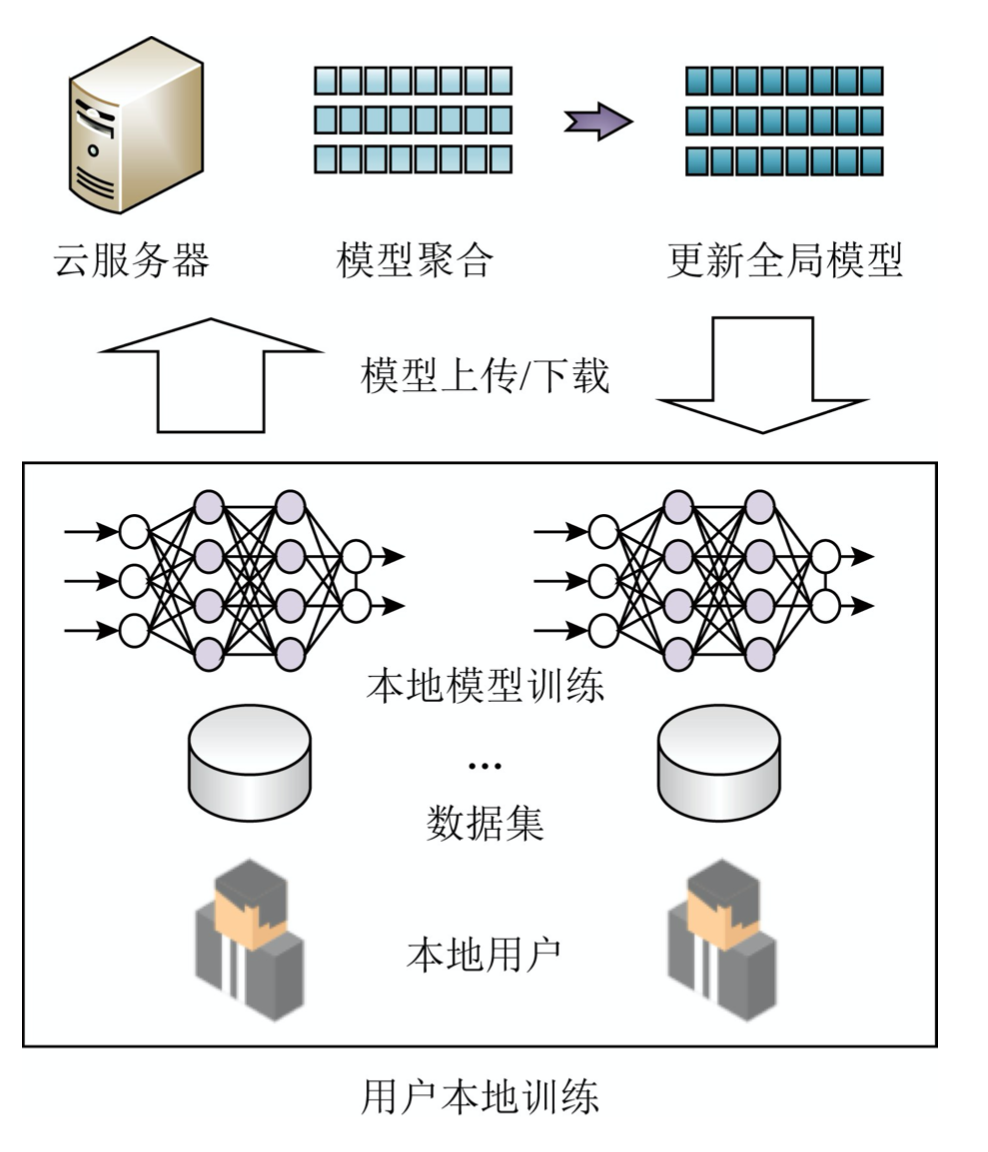
\includegraphics[scale=0.5]{fig2/C1/联邦学习训练模式}%联邦学习的系统架构
	\caption{联邦学习训练模型概览}
	\label{fig:联邦学习模型概况}	
\end{figure}

\section{安全性和隐私威胁}
尽管联邦学习解决了部分数据孤岛的问题,其本身还存在很多脆弱性和薄弱点。近年来,大量研究表明联邦学习机制仍然存在许多安全漏洞,这些漏洞可能被内部参与者和外部攻击者所利用,破坏联邦学习系统的安全性。由于联邦学习的框架并没有对参与方的资质进行校验、没有对模型的访问权加以约束,恶意的参与方可能将恶意的训练样本注入自己的本地模型中,影响全局模型的更新结果,导致最终的模型预测结果偏离,甚至全局模型不可用。此外,联邦学习也并没有考虑到对传递的参数进行保护,本地设备与中央服务器之间的通信信道有可能成为第三方窃取敏感信息的途径。本地设备上传到中央服务器的梯度本质是由模型和训练数据计算得到的函数,其中包含了关于本地训练数据的信息。攻击者可以从共享梯度中跟踪和获取参与者的隐私。综上,联邦学习的框架仍然存在本地训练数据泄漏、全局模型不可用等隐私问题。

图\ref{fig:联邦学习中的隐私威胁}大致概括了针对联邦学习隐私攻击的攻击者、攻击内容、攻击类型、攻击方式和攻击发生的时段。在联邦学习系统中,攻击方可能是内部攻击者,比如中央服务器、本地客户端。有一些恶意参与者作为本地客户端参与训练,修改本地的训练数据,注入一些有毒的数据,从而损害全局模型的准确性,操纵模型的预测结果;诚实但好奇的中央服务器通过观察本地客户端上传的梯度更新,篡改训练过程,并控制参与者对全局参数的视图。外部攻击者通过本地客户端与中央服务器之间的通信信道发起攻击,通过客户端上传的参数恶意的窃取用户的训练数据来生成样本原型。内部攻击通常比外部攻击更强,因为敌手拥有关于模型架构和内部参数的信息。

\begin{figure}[!hbt]
\centering
	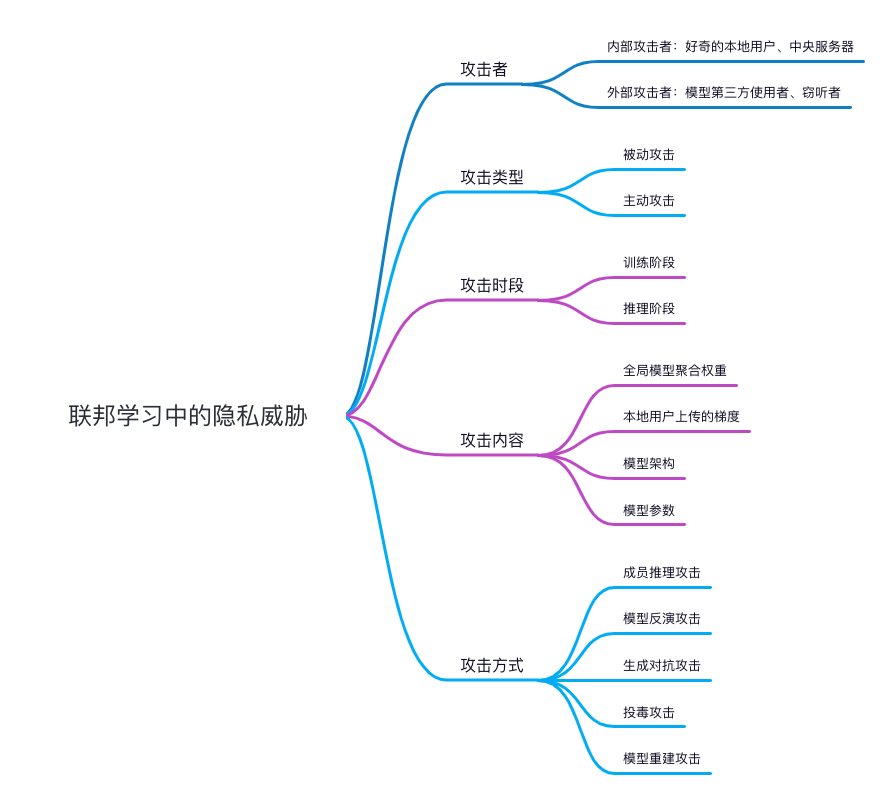
\includegraphics[scale=0.38]{fig2/C1/联邦学习中的隐私威胁}%联邦学习的系统架构
	\caption{针对联邦学习的隐私攻击}
	\label{fig:联邦学习中的隐私威胁}	
\end{figure}

针对联邦学习的攻击方式包括投毒攻击、模型反演攻击、成员推理攻击和生成对抗网络攻击等。

投毒攻击:投毒攻击通常发生在联邦学习的训练阶段。在联邦学习中,本地客户端在各自的设备上进行模型训练,将得到的训练参数上传给中央服务器。因为训练参数不需要通过可信机构的检查,所以有一些攻击者将恶意的训练样本注入自己的本地模型中,影响全局模型的更新结果,导致最终的模型预测结果错误甚至全局模型不可用。投毒攻击的影响对于许多企业和行业来说可能是致命的,在医疗部门、航空部门或道路安全方面甚至会危及生命。Marcus Comiter\upcite{ref56}曾使用投毒攻击进行实验,通过对熊猫的图像样本注入微小的恶意数据,导致算法预测结果发生重大变化,将熊猫识别为长臂猿。

模型反演攻击:当攻击者只能黑盒访问联邦模型时,攻击者仍然可以通过联邦学习系统提供的应用程序接口(Application programinterface,API)访问系统模型,通过向系统模型发送训练数据,获得所有表示类的预测标签和置信度信息,根据类标签和置信度数据重新建模,还原出目标模型的训练数据\upcite{ref11}。即使攻击者不清楚联邦模型的内部信息(训练参数、训练数据、模型结构等),依然可以通过API逆向反演获得所有预测数据的置信数据,由于置信信息代表了特征向量和标签类的关联性,攻击者将特征向量做为输入信息,对某一标签类进行分类或者回归得到置信度信息,其中置信度最高的类即为目标模型的目标类之一。

成员推理攻击:给定一个深度学习模型和一条数据样本(攻击者可以获取的知识范围),成员推理攻击旨在确定样本是否为用于构建此深度学习模型的训练集成员。例如,一个医疗机构根据基因型数据提供疾病预测的服务。假设保险公司持有某个客户A的基因型数据,通过对该疾病预测服务进行成员推理攻击,推断出A是否为某种疾病标签的成员样本,该公司就可以收取更多的费用以谋利。Shokri等人采用样本正确标签和目标模型预测的结果作为输入,通过影子学习的技术构建与目标模型的训练数据相近的数据集\upcite{ref13}。针对每一种数据样本,攻击者随机初始化一些数据记录作为影子模型的训练集数据。然后将此数据记录喂给目标模型得到预测向量,将所得的预测向量以及样本标签喂入攻击模型得到二分类的结果,达到推断任意样本是否在训练集中的目的。

生成对抗网络攻击:攻击者伪装成正常的用户参与联邦学习的训练,通过生成对抗网络(Generative Adversarial Networks,GAN)模型获得其他本地用户的训练数据。首先,攻击者在本地训练一个生成器网络和判别器网络,两者以零和博弈的思想进行对立训练,形成对抗生成式深度学习网络。生成器用来生成目标模型的伪样本,判别器被训练来区分图像是来自原始数据库还是由GAN生成的。攻击者将生成器生成的样本标记为"fake"类上传至全局模型,中央服务器通过聚合所有参与者上传的数据得到全局参数,攻击者通过基于假数据集的正常正向和反向计算获得假梯度,通过最小化假梯度和真实梯度之间的损失,反复优化假样本和标签,获得目标类的隐私数据。由于判别器参与了全局模型的训练,相当于在拥有该样本的用户训练数据上训练判别器,使得生成器有能力构造出与真实样本相似的伪样本。

\section{国内外研究现状}
随着针对联邦学习隐私攻击的模型增多,越来越多的研究者开始关注如何在联邦学习中应用隐私保护机制以防御上述的攻击模型。安全多方计算、同态加密和扰动技术是最常见的提高联邦学习中的安全性和隐私性的技术。

安全多方计算(Secure Multi-Party Computation,SMC)是由姚期智在1982年提出的\upcite{ref16},多个参与者在不泄露各自隐私数据情况下共同完成某项计算任务。安全多方计算是解决多方协同计算问题的一种解决方案,它必须保证计算中各方信息的保密性、独立性和准确性。当前,安全多方计算领域常见的技术主要包括混淆电路、零知识证明、不经意传输和秘密共享等。安全多方计算保护联邦学习的重点是如何在没有可信第三方的情况下安全地计算联邦学习中的经验风险最小化函数。同时,每个参与者都不可以获得任何关于其他用户的信息,除了梯度的聚合结果。Bonawitz等人利用SMC设计了一个联邦学习隐私保护框架,通过秘密分享技术安全地汇总用户的梯度,服务器只能看到聚合完成之后的梯度\upcite{ref3},不能知道每个用户的私有的真实梯度值,并且对用户的退出具有鲁棒性。然而,他们的模型由于涉及到学习过程中的多轮计算交互,在联邦学习通信回合数很大的情况下会导致通信性能大幅下降。

同态加密(Homomorphic Encryption,HE)是一种加密形式,允许第三方直接对密文进行算术运算\upcite{ref10}。在密文上进行计算后得到的结果进行解密,与明文上进行相同计算操作得到的结果是一致的。同态加密分为加法同态加密、乘法同态加密和全同态加密。同态加密保护联邦学习的隐私性主要通过将本地用户训练所得的梯度信息进行加密后上传至中央服务器,防止服务器对本地客户端上传的权重进行逆向工程从而反推出训练数据,确保每个客户端对全局模型的更改都保持隐藏状态。因为服务端接收的是本地客户端通过同态加密算法处理后的数据,这种模型的安全性是以服务器上的计算成本为代价的,加密场景的高计算复杂度会严重降低联邦学习的计算性能。 此外,由于需要传输公钥和秘钥也会增加额外的通信成本。Phong等人\upcite{ref23}提出了一个基于加法同态加密的联邦学习隐私保护方案,中央服务器可以根据同态操作,用加密的本地梯度更新全局模型参数。然而在基于联邦学习的系统中,有许多分布式设备(如智能手机和物联网设备)参与其中,用于解密的同一私钥需要分布到各个客户端,一旦持有相同秘钥的用户相互串通,将无法保证用户的数据隐私。

扰动技术的关键思想是在原始数据中加入噪声,使加躁后的数据与原始数据在统计特征上无法区分。三种广泛使用的扰动技术包括差分隐私、加法性扰动和乘法性扰动。差分隐私(Differential Privacy,DP)技术是基于概率统计模型来量化
数据集实例的隐私信息被披露的程度\upcite{ref75},其主要原理是向数据添加噪音,或使用概括方法来掩盖某些敏感属性\upcite{ref14},使至多相差1条数据的2个数据集的查询结果概率不可区分,以保护用户的隐私。差分隐私的优势在于其保护数据集所需要的隐私成本可以被量化,在通信效率和计算性能方面与明文计算相差不大。许多公司已经广泛采用差分隐私保护其联邦学习模型,包括谷歌、苹果、Uber、微软和LinkedIn。

在联邦学习框架应用差分隐私实现隐私保护基本可以分为两种方式:在本地模型训练阶段部署差分隐私;在全局参数聚合阶段部署差分隐私。

联邦学习中的本地用户进行模型训练的过程都可以看作是一次深度学习的过程。在深度学习中,差分隐私可以作为一种局部隐私保护方案来保护用户梯度的隐私。Song等人提出了一个$\left(\epsilon_{c}+\epsilon_{d}\right)$-差分隐私版本的随机梯度下降算法(DP-SGD),在本地模型的每一次迭代过程中对梯度添加高斯噪声,并通过差分隐私的组合性和隐私放大效果,得到完全隐私损失的上界\upcite{ref47}。然而,DP-SGD与SGD 相比严重降低了模型的准确率。当差分隐私提供的隐私保护强度增加时,在MNIST数据集上进行逻辑回归的训练和验证的损失率迅速增加。

Shokri等人\upcite{ref45}提出了一种选择性参数共享的差分隐私保护方案,通过对用户本地梯度绝对值进行排序,选择绝对值排名较大的梯度元素添加拉普拉斯噪声后参与联邦平均,然而随着模型迭代次数的增加,差分隐私的应用会导致模型的可用性下降。Choudhury等人\upcite{ref79}通过在联邦学习框架中应用分布式差分隐私机制,在两个真实的世界健康数据集上分析了不同的隐私预算对联邦模型性能的影响。他们给出的实验结果说明虽然差分隐私提供了一个强大的隐私水平,但是随着模型的通信回合数上升,整体隐私成本增加,模型性能大幅下降。

Geyer等人\upcite{ref48}研究发现与集中式学习相比,联邦学习中的梯度在整个训练过程中对噪声和批量大小具有不同的敏感度。他们的方案通过隐藏客户端的参与信息,实现客户层面的差分隐私,在分布式训练的过程中根据各个用户的隐私设置动态调整差分隐私的隐私参数,降低全局模型的性能损失。Truex等人\upcite{ref49}将差分隐私和同态加密技术相结合,在每个本地设备训练所得的权重上添加噪声后再使用同态加密技术进行加密,发送给中央服务器。中央服务器根据运算的同态性对加密后的数据进行聚合,更新全局参数。虽然通过差分隐私和同态加密加强了本地数据的隐私性,但是计算成本较高。

然而,Kang Wei等人\upcite{ref80}表示,Geyer\upcite{ref48}和Truex\upcite{ref49}的工作没有考虑到本地参数上传阶段的隐私保护,在向服务器上传训练结果时,客户的私人信息有可能被隐藏的敌手所截获。此外,这两篇文章缺乏对隐私性、收敛性能的具体分析。Kang Wei等人提出了提出了一个基于全局$(\epsilon, \delta)$-DP概念的新框架,对本地参数上传通道和全局参数下载通道定义不同的差分隐私要求,并在本地客户端和中央服务器采用不同的隐私参数添加高斯噪声。通过分析联邦学习模型损失函数的收敛界限,得出了以下结论:(1)模型的隐私保护水平越高,收敛性能越差;(2)在相同的隐私保护水平下,增加客户端的数量可以提高收敛性能;

总的来说,安全多方计算基于复杂的计算协议,同态加密的运算成本非常高,而现有的差分隐私保护联邦学习的方案很难在实现强隐私保护的同时,维持原有模型的精度。当使用较低的隐私预算达到较强的隐私保护的效果,可能使得模型难以收敛,可用性大幅下降;当隐私保护水平太低时,无法防御生成对抗网络攻击。当前的联邦学习中的隐私保护方案还有许多不足,很难在模型效用、数据隐私保护、通信性能这三个方面都达到满意的效果。

\section{研究内容与论文结构}
\subsection{研究内容}
联邦深度学习通过分布式的协作学习使得各个参与方在无需传递和共享本地的数据资源的情况下训练一个共同的、强大的深度学习模型。与传统的集中式深度学习相比,联邦学习在一定程度上缓解了数据孤岛和隐私泄露的问题。然而许多研究表明联邦学习机制仍然存在许多安全漏洞。联邦参与方、好奇的中央服务器以及外部的恶意敌手都有可能通过模型权重、共享的梯度和通信信道对联邦模型发起攻击,窃取用户的本地训练数据,破坏模型的可用性。差分隐私是当前保护联邦学习隐私安全的前沿技术,其通过严格的统计框架提供隐私保证和隐私成本计算,使得加躁后的梯度不能泄露关于实体数据的敏感信息。与安全多方计算和同态加密等密码学技术相比,差分隐私保护联邦学习的方案在通信性能和计算性能方面与明文计算相差不大。本文主要针对联邦学习的成员推理攻击和生成对抗网络攻击,设计基于差分隐私和安全混洗的隐私保护方案,对共享的梯度和模型权重进行隐私保护。本文的具体研究内容如下:

\begin{enumerate}
\item [(1)]在联邦学习的本地模型训练过程中,在每一轮随机梯度下降算法中对梯度注入高斯噪声,以防御成员推理攻击。现有的差分隐私保护深度学习方案大多数是基于固定的模型参数和隐私设置,很难在模型可用性和数据隐私性之间达到平衡效果。为了更好的解决现有的差分隐私保护数据隐私的同时,模型可用性下降的问题,本文对梯度加躁和梯度裁剪算法进行了以下优化:第一,根据逐层关联传播算法,在神经网络的前向和反向传播过程中分解神经元对于模型输出的贡献率,根据贡献率分配相应的隐私预算。保持整体的隐私预算不变,对于模型输出影响更大的梯度上添加较少的噪声,以减少梯度加躁对于模型可用性的影响。第二,在随机梯度下降算法的迭代过程中,根据之前训练所得梯度的统计特征,动态调整梯度裁剪阈值,尽可能的保留梯度中的有效信息。第三,本文采用“Moments Accountant”机制分析加噪累积产生的隐私预算,使得隐私损失的计算更加精确。

\item [(2)]当联邦学习中的用户数量达到千万量级时,在本地设备的模型训练上采用差分隐私技术,对于聚合后的梯度平均估计误差能达到$O\left(\frac{\sqrt{d \log d}}{\epsilon \sqrt{m}}\right)$。如果在迭代训练过程中的每一次迭代都应用本地差分隐私,隐私损耗就会成倍累积,从而导致聚合参数上的噪声溢出,影响全局模型的发布结果,增加了通信成本。为了解决这一问题,本文对基于本地差分隐私的联邦学习隐私保护方案进行了以下优化:第一,基于指数机制的打分函数和稀疏向量的思想对梯度进行采样扰动,相比本地差分隐私而言降低了计算复杂度;第二,在联邦学习中动态的调整客户端采样率,使用指数衰减率来递减训练过程中的采样率,在相同的通信回合下降低整体的通信成本;第三,在中央服务器和本地设备之间引入混洗器。混洗器将所有客户上传的加密数据集合中的向量元素进行拆分和随机置换,得到一个无序的消息集合。混洗和采样的操作达到了双重的隐私放大效应,从 $\left(\epsilon_{c}+\epsilon_{l}\right)$的本地差分隐私放大至 $\bar{\epsilon} $-中央差分隐私。在本地设备添加更少的噪声,而在中央服务器上达到相同的隐私保护效果,兼顾隐私保护能力与模型可用性。

\end{enumerate}

\subsection{论文结构}
本文一共五个章节,主要内容的组织安排如图所示:

第一章介绍了联邦学习的研究背景和存在的隐私威胁,并具体阐述了针对联邦学习的差分隐私保护的研究现状与发展方向,最后介绍了本文的相关工作和贡献。

第二章详细介绍了关于本文研究内容的基础知识,包括联邦学习的工作流程,差分隐私的基本概念和定理、神经网络的基本结构和训练算法。

第三章是基于本地自适应差分隐私保护联邦学习的共享梯度。首先,在引言部分介绍了差分隐私保护深度学习算法的四种扰动方式,主要针对梯度扰动分析了前人方案的不足之处,接着提出了本文所设计方案的两个创新点,依次详细的描述了梯度的自适应加躁算法和梯度的自适应裁剪算法的设计思路和实现流程。将梯度自适应的加躁和裁剪算法应用在随机梯度下降算法中,得到本地模型训练的核心算法,并结合MA机制分析总隐私损失。最后,我们通过三方面的实验对本地自适应差分隐私保护方案进行了全面的评估:其一,分析噪声水平、裁剪阈值、隐藏层数量这些参数对模型分类准确率影响;其二,与非隐私的SGD、前人提出的差分隐私SGD方案,比较各个方案在相同隐私预算的情况下模型分类所能达到的准确率和模型收敛速度;其三,针对部署了本地自适应差分隐私的联邦学习模型训练成员推理攻击模型,评估隐私保护效用。

第四章针对高维聚合场景下噪声成倍累积的问题,设计了Top-K梯度安全混洗算法。首先,定义了威胁模型和隐私表述,描绘了基于安全混洗的联邦学习模型框架,依次详细的描述了本地top-K梯度采样算法、客户端动态采样算法和梯度混洗算法的设计思路和实现流程。接着,证明了采样和混洗算法实现了$\left(\epsilon_{c}+\epsilon_{l}\right)$-本地差分隐私到 $\bar{\epsilon} $-中央差分隐私的隐私放大效用。最后,我们通过三方面的实验对Top-K梯度安全混洗算法进行了全面的评估:其一,分析客户端数量$N$、梯度选择的比率、客户端采样比$f_{r}$和最大聚合次数对于模型分类准确率的影响;其二,与非隐私的SGD、前人提出的差分隐私SGD方案进行对比实验,评估指标为模型分类准确率和通信性能;其三,针对部署了Top-K梯度安全混洗算法的联邦学习模型训练生成对抗网络攻击模型,评估隐私保护效用。

第五章是对文本的工作内容的总结和未来研究方向的展望。首先对本文的研究内容进行了概括,并总结了现有方案的不足之处,之后对未来的研究和改进方向进行了展望。

\section{本章小结}
这一章节为绪论,首先介绍了联邦学习的研究背景和存在的隐私威胁,并具体阐述了针对联邦学习的差分隐私保护的研究现状与发展方向,最后介绍了本文的相关工作、贡献和论文的组织结构。

